%% abtex2-modelo-projeto-pesquisa.tex, v-1.9.6 laurocesar
%% Copyright 2012-2016 by abnTeX2 group at http://www.abntex.net.br/ 
%%
%% This work may be distributed and/or modified under the
%% conditions of the LaTeX Project Public License, either version 1.3
%% of this license or (at your option) any later version.
%% The latest version of this license is in
%%   http://www.latex-project.org/lppl.txt
%% and version 1.3 or later is part of all distributions of LaTeX
%% version 2005/12/01 or later.
%%
%% This work has the LPPL maintenance status `maintained'.
%% 
%% The Current Maintainer of this work is the abnTeX2 team, led
%% by Lauro César Araujo. Further information are available on 
%% http://www.abntex.net.br/
%%
%% This work consists of the files abntex2-modelo-projeto-pesquisa.tex
%% and abntex2-modelo-references.bib
%%

% ------------------------------------------------------------------------
% ------------------------------------------------------------------------
% abnTeX2: Modelo de Projeto de pesquisa em conformidade com 
% ABNT NBR 15287:2011 Informação e documentação - Projeto de pesquisa -
% Apresentação 
% ------------------------------------------------------------------------ 
% ------------------------------------------------------------------------


\documentclass[
	% -- opções da classe memoir --
	12pt,				% tamanho da fonte
 	%openright,			% capítulos começam em pág ímpar (insere página vazia caso preciso)
 	oneside,
 	%twoside,			% para impressão em recto e verso. Oposto a oneside
	a4paper,			% tamanho do papel. 
	% -- opções da classe abntex2 --
	%chapter=TITLE,		% títulos de capítulos convertidos em letras maiúsculas
	%section=TITLE,		% títulos de seções convertidos em letras maiúsculas
	%subsection=TITLE,	% títulos de subseções convertidos em letras maiúsculas
	%subsubsection=TITLE,% títulos de subsubseções convertidos em letras maiúsculas
	% -- opções do pacote babel --
	english,			% idioma adicional para hifenização
	french,				% idioma adicional para hifenização
	spanish,			% idioma adicional para hifenização
	brazil,				% o último idioma é o principal do documento
	]{abntex2}

% ---
% PACOTES
% ---

% ---
% Pacotes fundamentais 
% ---
\usepackage{lmodern}			% Usa a fonte Latin Modern
\usepackage[T1]{fontenc}		% Selecao de codigos de fonte.
\usepackage[utf8]{inputenc}		% Codificacao do documento (conversão automática dos acentos)
\usepackage{indentfirst}		% Indenta o primeiro parágrafo de cada seção.
\usepackage{color}				% Controle das cores
\usepackage{graphicx}			% Inclusão de gráficos
\usepackage{microtype} 			% para melhorias de justificação

% ---

% ---
% Pacotes adicionais, usados apenas no âmbito do Modelo Canônico do abnteX2
% ---
\usepackage{lipsum}				% para geração de dummy text
% ---

% ---
% Pacotes de citações
% ---
\usepackage[brazilian,hyperpageref]{backref}	 % Paginas com as citações na bibl
\usepackage[alf]{abntex2cite}	% Citações padrão ABNT

% --- 
% CONFIGURAÇÕES DE PACOTES
% --- 

% ---
% Configurações do pacote backref
% Usado sem a opção hyperpageref de backref
\renewcommand{\backrefpagesname}{Citado na(s) página(s):~}
% Texto padrão antes do número das páginas
\renewcommand{\backref}{}
% Define os textos da citação
\renewcommand*{\backrefalt}[4]{
	\ifcase #1 %
		Nenhuma citação no texto.%
	\or
		Citado na página #2.%
	\else
		Citado #1 vezes nas páginas #2.%
	\fi}%
% ---


% ---
% Informações de dados para CAPA e FOLHA DE ROSTO
% ---
\titulo{EducaLar - Aplicativo que conecta quem tem o conhecimento a quem precisa}
\autor{Caio Henrique Machado de Oliveira - 16101023 \\Karen Silva Santos - 16101845\\Lucas Góes - 16101762\\Lucas Magrini - 16100586\\Ricardo Aparecido Bezerra Elias da Silva - 15203158}
\local{Osasco}
\data{2018}
\instituicao{%
  Centro Universitário UNIFIEO
  \par
  Engenharia da Computação
  \par
  Engenharia de Software II}
\tipotrabalho{Tese (Doutorado)}
% O preambulo deve conter o tipo do trabalho, o objetivo, 
% o nome da instituição e a área de concentração 
\preambulo{Projeto de criação de um aplicativo mobile utilizando os conceitros de Engenharia de Software abordados em sala de aula.}
% ---

% ---
% Configurações de aparência do PDF final

% alterando o aspecto da cor azul
\definecolor{blue}{RGB}{41,5,195}

% informações do PDF
\makeatletter
\hypersetup{
     	%pagebackref=true,
		pdftitle={\@title}, 
		pdfauthor={\@author},
    	pdfsubject={\imprimirpreambulo},
	    pdfcreator={LaTeX with abnTeX2},
		pdfkeywords={abnt}{latex}{abntex}{abntex2}{projeto de pesquisa}, 
		colorlinks=true,       		% false: boxed links; true: colored links
    	linkcolor=blue,          	% color of internal links
    	citecolor=blue,        		% color of links to bibliography
    	filecolor=magenta,      		% color of file links
		urlcolor=blue,
		bookmarksdepth=4
}
\makeatother
% --- 

% --- 
% Espaçamentos entre linhas e parágrafos 
% --- 

% O tamanho do parágrafo é dado por:
\setlength{\parindent}{1.3cm}

% Controle do espaçamento entre um parágrafo e outro:
\setlength{\parskip}{0.2cm}  % tente também \onelineskip

% ---
% compila o indice
% ---
\makeindex
% ---

% ----
% Início do documento
% ----
\begin{document}

% Seleciona o idioma do documento (conforme pacotes do babel)
%\selectlanguage{english}
\selectlanguage{brazil}

% Retira espaço extra obsoleto entre as frases.
\frenchspacing 

% ----------------------------------------------------------
% ELEMENTOS PRÉ-TEXTUAIS
% ----------------------------------------------------------
% \pretextual

% ---
% Capa
% ---
\imprimircapa
\imprimirfolhaderosto

\pdfbookmark[0]{\contentsname}{toc}
\tableofcontents*
\cleardoublepage
% ---
\textual

% ----------------------------------------------------------
% Introdução
% ----------------------------------------------------------
\include{justificativa}
\include{objetivos}
%\include{conhecimento}
\chapter[Recursos]{Recursos}

\section[Hardware]{Hardware}

Quanto aos equipamentos que serão utilizados pela equipe, abaixo a relação e seu custo para o projeto.

\begin{figure}[htb]
	%\caption{\label{gantt}Placa Wiring S}
	\begin{center}
	    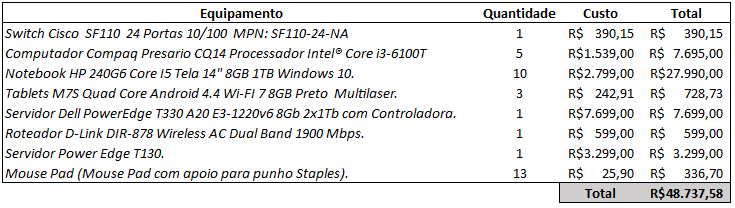
\includegraphics[scale=0.7]{figuras/custoHardware}
	\end{center}
	%\legend{Fonte: Site da 3GPP}
\end{figure}

\section[Software]{Software}

Utilizaremos 14 softwares distribuídos conforme tabela abaixo

\begin{figure}[htb]
	%\caption{\label{gantt}Placa Wiring S}
	\begin{center}
	    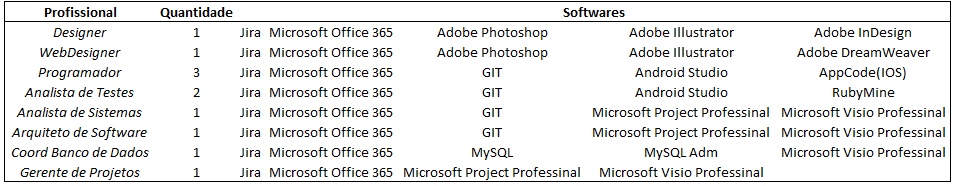
\includegraphics[scale=0.6]{figuras/relacaoSoftwares}
	\end{center}
	%\legend{Fonte: Site da 3GPP}
\end{figure}

Quanto ao custo de cada software, abaixo tabela com licença e custos por mês e/ou usuários.

\begin{figure}[!htb]
	%\caption{\label{gantt}Placa Wiring S}
    \begin{center}
	    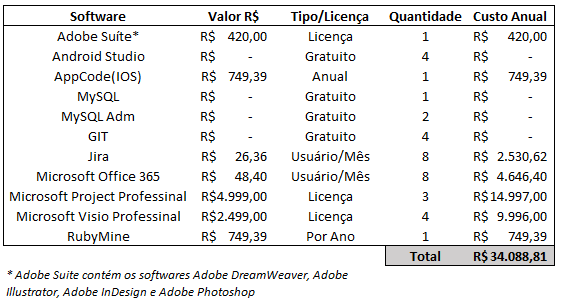
\includegraphics[scale=0.6]{figuras/custoSoftwares}
	\end{center}
	%\legend{Fonte: Site da 3GPP}
\end{figure}

    

% Colocar valores 
\chapter[Equipe]{Equipe}

Para a criação do aplicativo montaremos uma equipe com 12 pessoas, profissionais da área de tecnologia, que trabalharão em pequenas partes do desenvolvimento. O conjunto das partes resultará no EducaLar.


\begin{figure}[htb]
	%\caption{\label{gantt}Placa Wiring S}
	\begin{center}
	    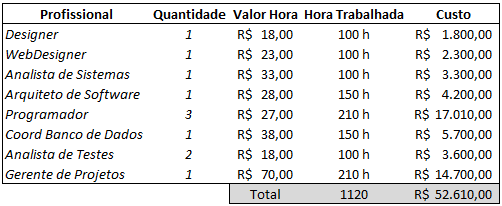
\includegraphics[scale=0.9]{figuras/tabelaCustos}
	\end{center}
	%\legend{Fonte: Site da 3GPP}
\end{figure}

%\begin{alineas}
%    \item Um Designer (ou \emph{Front End Designer}) %que é a pessoa %responsável por elaborar o desenho das interfaces do aplicativo.
%    \item Um Web designer %que vai ser responsável por aplicar o layout %projetado anteriormente.
%    \item Um Analista de sistemas %que vai ser responsável por %compreender a necessidade de negócio do cliente e especificar por %escrito o que precisa ser feito no projeto.
%    \item Um Arquiteto de software %que vai analisar as necessidades do %projeto e define a arquitetura técnica que melhor se encaixa no %projeto.
%    \item Cinco desenvolvedores/programadores %que vai transformar as %especificações de negócio do aplicativo em código sendo responsáveis %por 50 \% do esforço total do projeto de desenvolvimento e manutenção %do aplicativo.
%    \item Um analista de banco de dados %que vai tratar adequadamente %do grande volume de dados.
%    \item Um analista de testes %que vai fazer a validação do %aplicativo analisando todo sistema e vendo se não há erros %(\emph{bugs}) no aplicativo.
%    \item Gerente de projetos %que cria e acompanha o cronograma do %projeto, dando as diversas tarefas para os profissionais
%\end{alineas}
\chapter[Metas]{Metas}

%O projeto conta com quatro grandes metas principais, passando de criação e desenvolvimento até a parte de lançamento e estabilidade do aplicativo. 

%Como meta inicial, após a elaboração do plano de desenvolvimento do software, faremos a criação e desenvolvimento do aplicativo, parte principal do projeto, buscando robustez já na primeira versão.
% Está vago

%Como segundo passo, trazendo a tarefa que por muitos é dada como mais importante, fazer o teste do aplicativo que vai analisar os mínimos detalhes e possíveis falhas, possibilitando entregar uma versão o mais estável possível. 

%Fazer a divulgação por meio de feiras de ensino, escolas, nas diversas redes sociais e nos sites de ensino, buscando levar o aplicativo não só para as pessoas que querem aprender, mas sim, as que querem ensinar.

%Por último, a tarefa de manter o aplicativo no ar, trabalhando e assegurando que o aplicativo ficará 24 horas disponível e funcional.

% Separar em tópicos
% Aprofundar mais
% Alguns termos estão razos

\section[Cronograma]{Cronograma}

% Como estamos falando de um aplicativo de médio porte, padronizando horário com aplicativos criados ele demoraria de 500 a 800 horas para ser desenvolvido. 

%---- Aqui vai uma tabela ----


O projeto levará 7 meses (1120 horas)

%---- Aqui vai uma tabela ----



\begin{figure}[htb]
	%\caption{\label{gantt}Placa Wiring S}
	\begin{center}
	    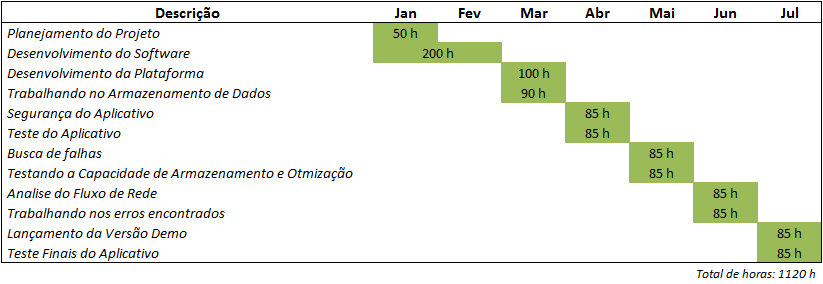
\includegraphics[scale=0.8]{figuras/diagramaGanttCrono}
	\end{center}
	%\legend{Fonte: Site da 3GPP}
\end{figure}

% Não está legal. Montar um cronograma \textit{like a} iniciação científica associando o tópico de metas


% Notas de Aula (CICLO DE VIDA)

% Prazos e Tarefas (Inicio, Desenvolvimento e Final) . Fase 1 discussão, planejamento, desenvolvimento planejamento.

% Cada etapa é uma tarefa. Cada tarefa tem um prazo. (HORAS)

%% CICLO
% Levantamento -> Análise - > Projeto -> Implementação -> Manutenção

% Requisito é etapa "Cada momento é um tempo, cada tempo é uma ação" (PROFESSORA)
\include{cronograma}
\chapter[Investimento]{Investimento}

Para a realização deste projeto o valor do investimento será de R\$ 140.000,00.

% Novo tópico para divulgação?
%    \section[Divulgação]{Divulgação} 
%        Optaremos pela divulgação em redes socias, através de páginas gerenciadas pelos membros da equipe. Para uma penetração maior, optaremos por anúncios em apps de educação, gerando um custo estimado de R\$ 5 mil / ano.




%    \section[Manutenção e Mantenabilidade]{Manutenção e Mantenibilidade}
%        Barry Boehm propõe que o custo de manutenção de um software é de \$ 1 mil por linha de código. Além disso temos os custos de servidores de software que podem girar em torno de R\$ 20 mil / ano.


\chapter[Risco]{Risco}

Identificamos os seguintes riscos para execução do projeto:

\begin{alineas}
    \item Capital inferior ao necessário, tendo que recorrer a redução de custos deixando assim um padrão inferior ao desejado.
    \item Desistência do projeto devido a problemas financeiros.
    \item Problemas de gestão / operação.
    \item Atrasos na entrega das etapas.
    \item Problemas técnicos com aparelhos.
    \item Concorrência.
    \item Indisponibilidade de mercado para atuação.
\end{alineas}

% Professora quer mais detalhes em cada tópico


\phantompart
\postextual
\phantompart
\printindex

\end{document}
